\begin{frame}{Piet}
    % \begin{columns}

	% 	\begin{column}{.5\hsize}
			\begin{itemize}
				\myitem David Morgan-Mar, 2003
				\myitem Zainspirowany abstrakcyjną twórczością Piet'a Mondrian'a
				\myitem Kodem źródłowym jest dwuwymiarowa bitmapa
                \myitem W zależności od różnicy kolorów, ruchomy wskaźnik uruchamia różne komendy i korzysta ze stosu
			\end{itemize}
		% \end{column}

        % \begin{column}{.5\hsize}
			% 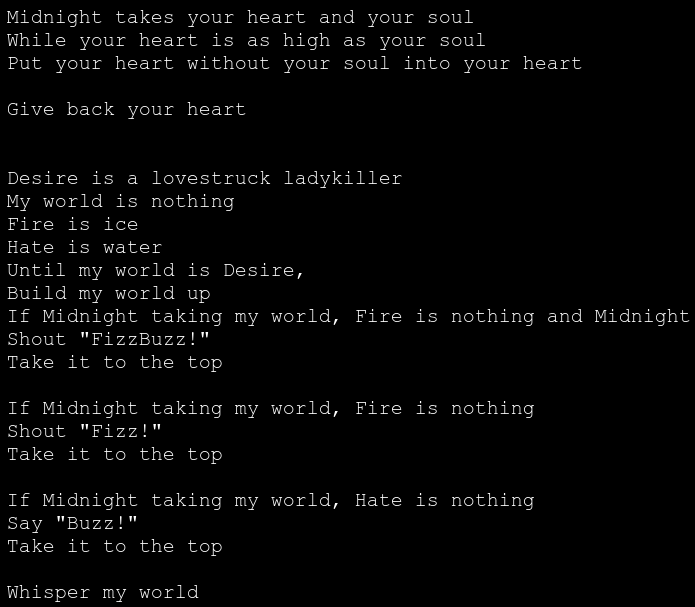
\includegraphics[height=7cm]{figures/rockstar1.png}
		% \end{column}

	% \end{columns}
    \begin{columns}
        \begin{column}{.5\hsize}
            \begin{figure}
                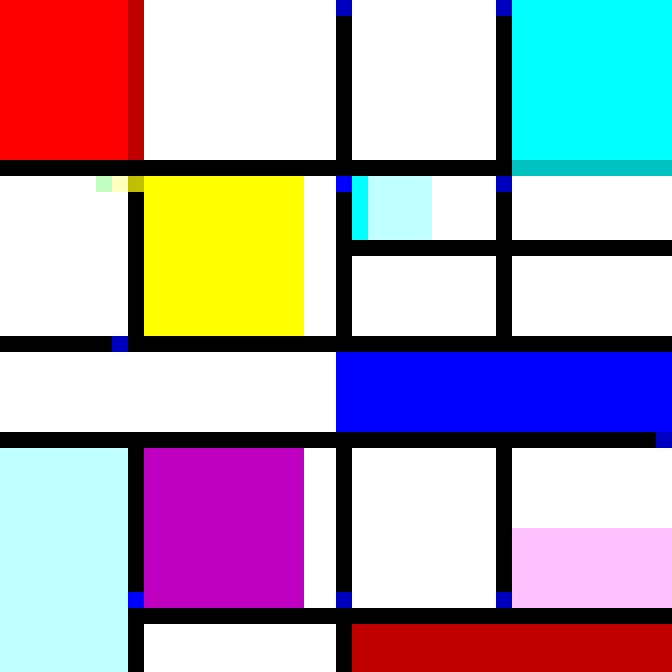
\includegraphics[height=2cm]{figures/piet_piet.png}
                \caption*{\scriptsize Program drukujący ,,Piet''{\color{blue} \hyperlink{frame:przypisy}{(7)}}}
            \end{figure}
        \end{column}
        \begin{column}{.5\hsize}
            \begin{figure}
                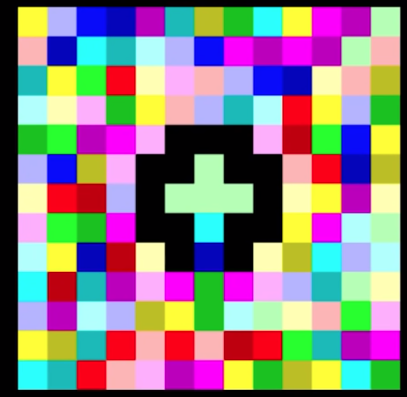
\includegraphics[height=2cm]{figures/piet_helloworld.png}
                \caption*{\scriptsize Program drukujący ,,Hello World!''{\color{blue} \hyperlink{frame:przypisy}{(7)}}}
            \end{figure}
        \end{column}
    \end{columns}


\end{frame}
